\epigraph{\textit{The business changes. Technology changes. The team changes. The team members change. Change is not the problem, per se, because change is going to happen; the problem, rather, is the inability to cope with change when it comes.}}{-- \textup{Kent Beck}}

During the early stages of the development, the first steps we followed were highly related to polishing and improving the solution described in the previous chapter. This was a challenging problem that resulted in a change in the project's direction, which will be detailed later.

\section{Technology stack}

As I've mentioned earlier, the purpose of this second solution was to improve what was already implemented. This way, we kept most of the stack untouched. The sole change was the replacement of GraphX with its DataFrame equivalent library named GraphFrames.

\begin{figure}[ht]
    \centering
    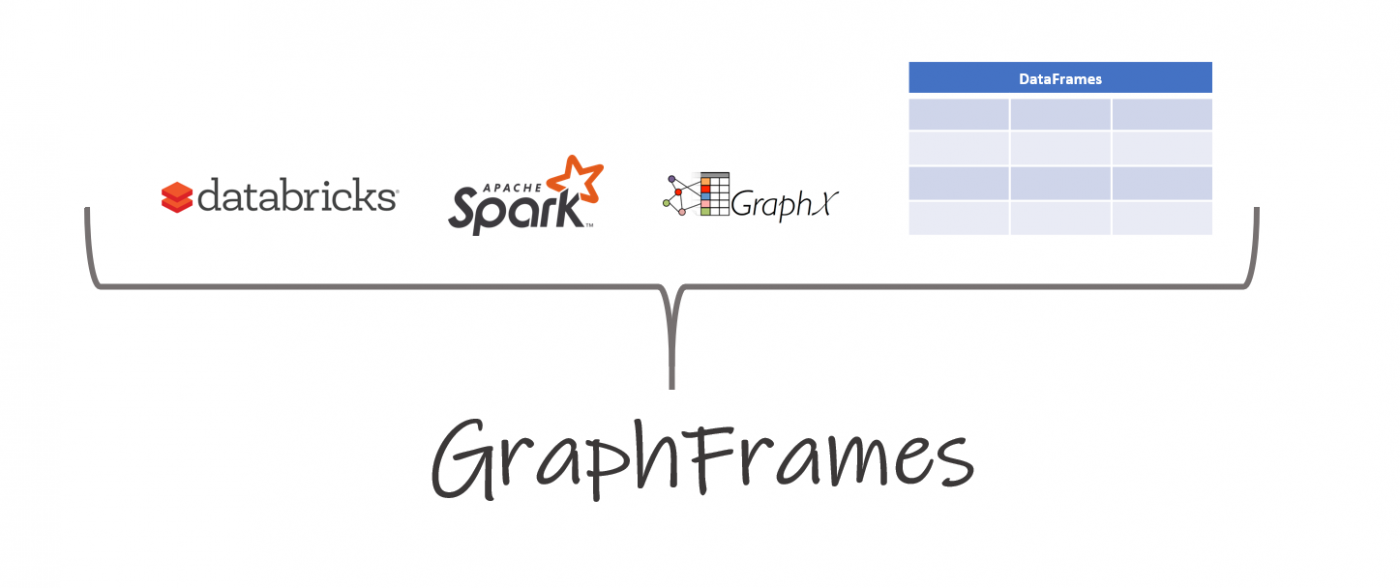
\includegraphics[width=.7\linewidth]{img/8-1_graphframes.png}
    \caption[Stack of the different technologies we are using for the second solution]{Stack of the different technologies we are using for the second solution\footnotemark}
\end{figure}

\footnotetext{\url{https://adatis.co.uk/graphframes/}}

\subsection{Row-based vs. column-based storage}

What we have seen thus far is one of the most common approaches for storing data: row-oriented databases. However, there is another approach that has been gaining traction during the past few years, namely, columnar storage. In the former, data is organized by records, keeping all the information related to a particular entity close to each other in memory. In the latter, data is organized by columns, keeping all the values for a particular attribute close to each other in memory. This is especially relevant when we are working with large amounts of data, as we can perform operations over a particular column without having to load the whole row -- for each entity -- into memory.

Row-oriented databases are the way to go when reading or writing entire rows is the most common operation. This is the case for \texttt{OLTP (Online Transaction Processing)} systems, where we are usually working with small amounts of data. On the other hand, column-oriented databases are the way to go when we are working with \texttt{OLAP (Online Analytical Processing)} systems, where we are usually working with large amounts of data, as we have said before. As an example, let's imagine we have a table with the following schema: \texttt{<ID, name, age, address>}. Having that said, let us assume we have the following data in our table:

\begin{table}[ht]
    \centering
    \begin{tabular}{|c|c|c|c|}
        \hline
        \rowcolor[HTML]{EFEFEF}
        \texttt{ID} & \texttt{name} & \texttt{age} & \texttt{address}            \\ \hline
        1           & John          & 25           & \textit{1234 Main St.}      \\ \hline
        2           & Jane          & 30           & \textit{5678 Main St.}      \\ \hline
        3           & Angel         & 23           & \textit{1234 Secondary St.} \\ \hline
        4           & Eve           & 23           & \textit{5678 Secondary St.} \\ \hline
    \end{tabular}
    \caption{Table with some data}
\end{table}

In a more traditional row-based database the data is stored by rows, such that the first column of a row will be next to the last attribute of the previous one. According to this, we will have the following layout in memory:

\begin{table}[ht]
    \centering
    \begin{tabular}{|c|c|}
        \hline
        \multicolumn{1}{|l|}{\cellcolor[HTML]{EFEFEF}}                                 & 1                           \\ \cline{2-2}
        \multicolumn{1}{|l|}{\cellcolor[HTML]{EFEFEF}}                                 & John                        \\ \cline{2-2}
        \multicolumn{1}{|l|}{\cellcolor[HTML]{EFEFEF}}                                 & 25                          \\ \cline{2-2}
        \multicolumn{1}{|c|}{\multirow{-4}{*}{\cellcolor[HTML]{EFEFEF}\textbf{Row 1}}} & \textit{1234 Main St.}      \\ \hline
        \multicolumn{1}{|l|}{\cellcolor[HTML]{EFEFEF}}                                 & 2                           \\ \cline{2-2}
        \multicolumn{1}{|l|}{\cellcolor[HTML]{EFEFEF}}                                 & Jane                        \\ \cline{2-2}
        \multicolumn{1}{|l|}{\cellcolor[HTML]{EFEFEF}}                                 & 30                          \\ \cline{2-2}
        \multicolumn{1}{|c|}{\multirow{-4}{*}{\cellcolor[HTML]{EFEFEF}\textbf{Row 2}}} & \textit{5678 Main St.}      \\ \hline
        \multicolumn{1}{|l|}{\cellcolor[HTML]{EFEFEF}}                                 & 3                           \\ \cline{2-2}
        \multicolumn{1}{|l|}{\cellcolor[HTML]{EFEFEF}}                                 & Angel                       \\ \cline{2-2}
        \multicolumn{1}{|l|}{\cellcolor[HTML]{EFEFEF}}                                 & 23                          \\ \cline{2-2}
        \multicolumn{1}{|c|}{\multirow{-4}{*}{\cellcolor[HTML]{EFEFEF}\textbf{Row 3}}} & \textit{1234 Secondary St.} \\ \hline
        \multicolumn{1}{|l|}{\cellcolor[HTML]{EFEFEF}}                                 & 4                           \\ \cline{2-2}
        \multicolumn{1}{|l|}{\cellcolor[HTML]{EFEFEF}}                                 & Eve                         \\ \cline{2-2}
        \multicolumn{1}{|l|}{\cellcolor[HTML]{EFEFEF}}                                 & 23                          \\ \cline{2-2}
        \multicolumn{1}{|c|}{\multirow{-4}{*}{\cellcolor[HTML]{EFEFEF}\textbf{Row 4}}} & \textit{5678 Secondary St.} \\ \hline
    \end{tabular}
    \caption{Row-based storage}
\end{table}

This way, writing to a row store is an optimized operation. To put it into perspective, let me show you an example. Let's assume we want to add a new record to our table, namely, \texttt{<5, Bob, 25, 1234 Main St.>}. In this case, we will just have to append the new record at the end of the table, as we can see in figure \ref{table:row-based-storage}. Note that the ellipsis stands for the rest of the table, which is not shown for the sake of simplicity.

\begin{table}[ht]
    \centering
    \begin{tabular}{|c|c|}
        \hline
        \multicolumn{2}{|c|}{$\cdots$}                                                    \\ \hline
        \cellcolor[HTML]{EFEFEF}                                 & 5                      \\ \cline{2-2}
        \cellcolor[HTML]{EFEFEF}                                 & Bob                    \\ \cline{2-2}
        \cellcolor[HTML]{EFEFEF}                                 & 25                     \\ \cline{2-2}
        \multirow{-4}{*}{\cellcolor[HTML]{EFEFEF}\textbf{Row 5}} & \textit{1234 Main St.} \\ \hline
    \end{tabular}
    \caption{Inserting a new record in row-based storage}
\end{table}
\label{table:row-based-storage}

This proves that row-oriented storage is very efficient when we want to add new records to our table. However, if we want to read a specific \textit{column}, we will have to read the entire table, which is not performant. For example, if we want to read the \texttt{name} column, we will load all five rows into memory and then pull out the second attribute of each one of them. As you can see, this approach lacks efficiency as we are loading a lot of data that we are not going to use. To address this issue, column-based storage was designed. In this case, the data is stored by columns, such that all the elements of each row will be next to each other in memory. According to this, and following the same example as before, we will have the following disk layout:

\begin{table}[ht]
    \centering
    \begin{tabular}{|c|c|}
        \hline
        \cellcolor[HTML]{EFEFEF}                                   & 1                           \\ \cline{2-2}
        \cellcolor[HTML]{EFEFEF}                                   & 2                           \\ \cline{2-2}
        \cellcolor[HTML]{EFEFEF}                                   & 3                           \\ \cline{2-2}
        \multirow{-4}{*}{\cellcolor[HTML]{EFEFEF}\texttt{ID}}      & 4                           \\ \hline
        \cellcolor[HTML]{EFEFEF}                                   & John                        \\ \cline{2-2}
        \cellcolor[HTML]{EFEFEF}                                   & Jane                        \\ \cline{2-2}
        \cellcolor[HTML]{EFEFEF}                                   & Angel                       \\ \cline{2-2}
        \multirow{-4}{*}{\cellcolor[HTML]{EFEFEF}\texttt{name}}    & Eve                         \\ \hline
        \cellcolor[HTML]{EFEFEF}                                   & 25                          \\ \cline{2-2}
        \cellcolor[HTML]{EFEFEF}                                   & 30                          \\ \cline{2-2}
        \cellcolor[HTML]{EFEFEF}                                   & 23                          \\ \cline{2-2}
        \multirow{-4}{*}{\cellcolor[HTML]{EFEFEF}\texttt{age}}     & 23                          \\ \hline
        \cellcolor[HTML]{EFEFEF}                                   & \textit{1234 Main St.}      \\ \cline{2-2}
        \cellcolor[HTML]{EFEFEF}                                   & \textit{5678 Main St.}      \\ \cline{2-2}
        \cellcolor[HTML]{EFEFEF}                                   & \textit{1234 Secondary St.} \\ \cline{2-2}
        \multirow{-4}{*}{\cellcolor[HTML]{EFEFEF}\texttt{address}} & \textit{5678 Secondary St.} \\ \hline
    \end{tabular}
    \caption{Column-based storage}
\end{table}

This way, if we want to read a specific column, we will only have to read the one we are interested in. For example, if we want to read the \texttt{name} column, we will just retrieve the second one, which is much more efficient than reading the entire table. However, if we want to append a new record, we will have to add a new entry to the end of each column, leading to a slower insertion. For example, if we want to add the record \texttt{<5, Bob, 25, 1234 Main St.>} to our table, we will add the entries to each column as seen in figure \ref{tab:column_based}. Note that the ellipsis stands for the rest of the entries of each column, which are not shown for the sake of simplicity.

\begin{table}[ht]
    \centering
    \begin{tabular}{|c|c|}
        \hline
        \cellcolor[HTML]{EFEFEF}                                   & $\cdots$               \\ \cline{2-2}
        \multirow{-2}{*}{\cellcolor[HTML]{EFEFEF}\texttt{ID}}      & 5                      \\ \hline
        \cellcolor[HTML]{EFEFEF}                                   & $\cdots$               \\ \cline{2-2}
        \multirow{-2}{*}{\cellcolor[HTML]{EFEFEF}\texttt{name}}    & Bob                    \\ \hline
        \cellcolor[HTML]{EFEFEF}                                   & $\cdots$               \\ \cline{2-2}
        \multirow{-2}{*}{\cellcolor[HTML]{EFEFEF}\texttt{age}}     & 25                     \\ \hline
        \cellcolor[HTML]{EFEFEF}                                   & $\cdots$               \\ \cline{2-2}
        \multirow{-2}{*}{\cellcolor[HTML]{EFEFEF}\texttt{address}} & \textit{1234 Main St.} \\ \hline
    \end{tabular}
    \caption{Inserting a new record in column-based storage}
    \label{tab:column_based}
\end{table}

Putting this all together, row-based databases will be more efficient when performing operations such as \texttt{SELECT * FROM table WHERE id = 1}, as we only need to read the first row. On the other hand, columnar stores will be more efficient when performing operations such as \texttt{SELECT SUM(age) FROM table}, as we only need to read the third column. A typical use-case for row-based databases is systems where the most common operations are any of: \texttt{Create-Read-Update-Delete}. Following into this, row-based databases are commonly used in traditional DBMS such as \texttt{MySQL} or \texttt{PostgreSQL}; to name an example, row-oriented storage excels at \textit{e-commerce} applications where we are required to load whole rows into memory, that is, we may need to retrieve the name, description and price of every item in the shop, or in the case of having to perform frequent insertions to the database. On the other hand, a typical use-case for column-based databases is systems where the most common operations are aggregations and complex queries in general. Following into this, column-based databases are commonly used in data warehouses such as \texttt{Amazon Redshift} or \texttt{Google BigQuery}; to name an example, column-oriented storage excels at \textit{business intelligence} applications where we are required to perform aggregations over a particular column, more precisely, we may need to retrieve the total revenue of the shop, Which is the case for our solution. As we are performing aggregations over columns for each iteration of the Pregel model. This is why we decided to move from row-based to column-oriented storage.

\subsection{GraphFrames}

To continue with what we have been discussing so far, we will now introduce GraphFrames. As its name goes, \texttt{GraphFrames} is a package for Apache Spark providing support for DataFrame-based Graphs and operations over them. According to the introductory lines, the main goal of this stage of the development was to move our solution one step further in the abstraction level, from a solution based on RDDs to another based on DataFrames. From the ground up, we always believed RDDs weren't the go-to. What's more, RDDs are discouraged as they seem to be outdated in comparison to DataFrames and Datasets. More into this will be discussed in the next section. According to the description of the GraphFrames library, this API is similar to GraphX, except, instead of being built on top of RDDs, they are based on DataFrames. However, the fact that the Pregel implementation bundled in the GraphFrames API  has not been updated since 2018, makes us feel cautious about this approach.

\subsection{DataFrames and Datasets}

From Spark version 1.3 onwards, what was once known as SchemaRDDs are now referred to as DataFrames. That may give us an idea of what a DataFrame is. In that sense, they are RDDs provided some Schema for the data that is collected. With the help of this schema, DataFrames may be seen as rows with uniform structure: columns. Whereas RDDs are more akin to objects, DataFrames are closer to a table in a database. This is quite relevant, as managing schemas to describe the information allows us to perform operations over data in a more efficient manner when compared to using Java serialization. It is worth mentioning that from Spark version 2.0 onwards, DataFrames can be understood as a type alias for \texttt{Dataset[Row]}, as they merged both APIs. In that sense, Datasets can be seen as the combination of the best of both worlds: with the appearance of a Java object from the outside, but with the shape of a table in RDBMS internally.

We now have a clear vision of what a DataFrame is. The problem is that even though they provide some nice features for data wrangling: schemas allow us to establish contracts so consumers know exactly the shape of the data they are working with, they are not so nicely implemented currently. Not only Apache Spark has no official support for working with DataFrame-based Graphs: notice GraphFrames is required, but the variety of supported types is scarce: including primitive types and Dates. Long has been discussed in this sense, but nothing has changed since 2015\footnote{\url{https://issues.apache.org/jira/browse/SPARK-7768}}. To clarify this, let's put it into perspective.

\label{sec:encoders}
\subsubsection{Encoders and User-defined Types}

Working with simple data structures is a trivial task in Apache Spark. What is not so easy to handle are custom data types. If the DataFrame cannot implicitly retrieve an \texttt{Encoder}, the user will be required to provide one. This is needed for Spark SQL to infer the schemas of the data we are working with. The more complex the data structure, the harder it is for the programmer to write an appropriate serialization/deserialization mechanism. Notice how this solution is far from efficient as it is based on serialization for data storage and retrieval, something we were trying to avoid when we dropped the RDD-based solution. Another possibility could be writing your own \texttt{User-defined types}, which can be understood as \textit{wrappers} for the actual type. However, the amount of boilerplate code needed, and the complexity of the data to be stored prevents us from writing an appropriate solution.

As we have mentioned earlier, two main possible solutions arise for the problem of handling complex data: \textit{Custom encoders} and \textit{User-defined types}. It is a requirement for this solution not only to handle complex data but unsupported, as we are not only trying to store complex data structures but types that are not currently supported by the DataFrame API. This is a crucial argument against this DataFrame-based solution as we need to store URLs, which aren't currently backed by Spark SQL. The problem is that both of the provided solutions are inefficient. First, collection Encoders tend to act as bottlenecks in terms of performance. To follow up on this, storing non-standard objects in Spark is a mess\footnote{\url{https://stackoverflow.com/questions/36648128/how-to-store-custom-objects-in-dataset}}. The latest version of the framework supports primitive types and dates, as have already mentioned. The currently accepted solution in this sense consists of serializing objects using the \texttt{kryo} encoder which stores them as flat binary objects, preventing us from accessing concrete columns without deserializing the binary. This last matter is especially crucial as messaging in Pregel is built on top of aggregates over particular columns. Hence, we would need to serialize and deserialize every stored item for each iteration. Thus, a  complex and inefficient encoder is not the solution we need. See figure \ref{fig:wikibaseClassDiagram} for an expanded description of Wikibase's data model as implemented in WShEx.

\begin{code}[User-defined types as implemented in Apache Spark]
    \inputminted{scala}{code/listings/8-1_udt.scala}
\end{code}

As noted in the first line of the example above, the description of User-defined types is annotated as an unstable API meant for developers. This implies that in minor Spark versions, the API may change or be eliminated. The use of it is at the user's own risk. As a consequence, if we follow this approach, we will end up with an unstable solution. Not only that but the processes for serializing and deserializing, along with the SQL schema -- which is no longer inferred by Scala's reflection system -- should be explicitly defined. Having said that, by defining our User-defined types, we're only establishing the wrapper, and yet no relationship is established between the real object and the User-defined type in the eyes of Spark's engine. To deal with this, we have two options: annotating the class we want to encapsulate or explicitly registering it. The former requires that the programmer has access to the class being wrapped. An ineffective technique that has been superseded by the latter since Spark 2.0. What's striking here is that it took Spark developers 6 years to come up with an answer in this regard. The API for user-defined types is essentially unmaintained, and dealing with custom objects in Spark is the framework's weak point. More on this was covered in the previously mentioned issue\footnote{\url{https://issues.apache.org/jira/browse/SPARK-7768}}.

\begin{code}[Registration of an User-defined type in Apache Spark]
    \inputminted{scala}{code/listings/8-2_udtRegistration.scala}
\end{code}

The issue here is the complexity of the data structures we use. According to the design in figure \ref{fig:wikibaseClassDiagram}, storing both \texttt{Statements} and \texttt{Entities} presents two major challenges. To begin, as the items stored require a fixed structure and we would like to polymorphically treat \texttt{Properties} and \texttt{Items} -- both -- as \texttt{Entities}, we need a mapping to convert from an object-oriented model to the relational paradigm. In this regard, we suggest \textit{Single Table Inheritance}\footnote{\url{https://en.wikipedia.org/wiki/Single_Table_Inheritance}}; that is, using a single table containing all the fields of all the child classes. The issue here is that we would end up with a solution in which rows contain redundant data: as many \texttt{NULL} values as different fields in child classes that are not the actual type for a certain row. Although it is a straightforward approach, it is inefficient. Second, this technique leads to a circular dependency\footnote{\url{https://en.wikipedia.org/wiki/Circular_dependency}} in which \texttt{Entities} include many \texttt{LocalStatements} that hold \texttt{Qualifiers} that may enclose \texttt{Entities}. When you define a schema for this problem, you eventually wind yourself in an infinite recursion where \texttt{Entities} have \texttt{Entities}. In conclusion, User-defined types offer a poor solution that causes several challenging issues.

\begin{figure}[ht]
    \centering
    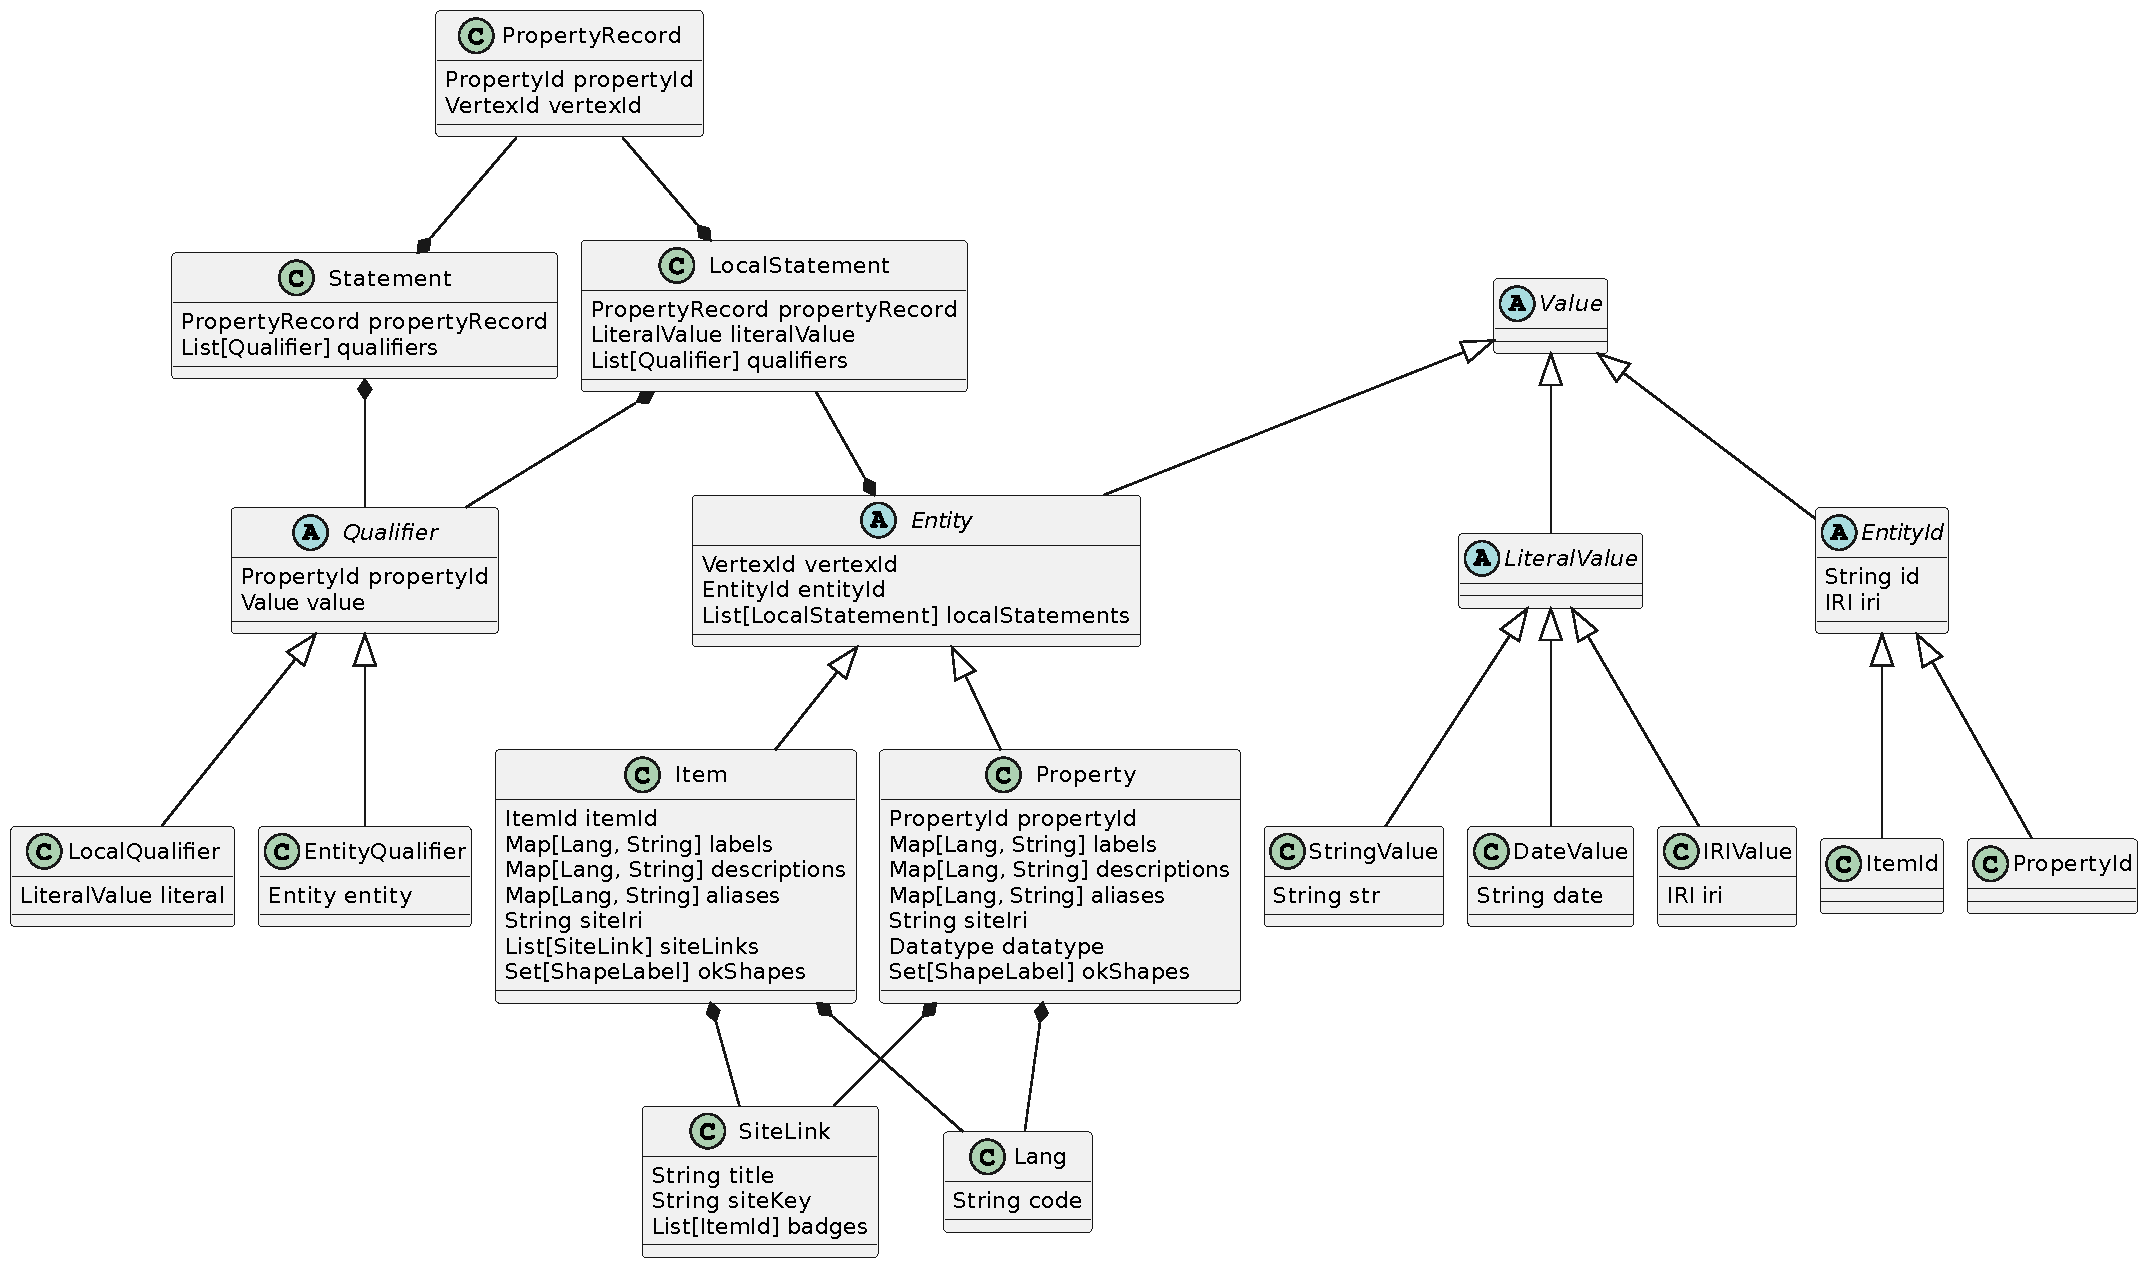
\includegraphics[width=\textwidth]{diagrams/8-1_wikibaseClassDiagram.pdf}
    \caption[Class diagram of the Wikibase data model as implemented in WShEx]{Class diagram of the Wikibase data model as implemented in WShEx\footnotemark}
    \label{fig:wikibaseClassDiagram}
\end{figure}
\footnotetext{\url{https://github.com/weso/shex-s}}

At this point, we can agree that we have ended up in a pitfall. This is, we have identified a challenge in storing intricate data structures in Spark. Additionally, we have examined the two primary approaches to tackle this issue and explained why they are unsuitable for our specific situation. An alternative approach is required, specifically, simplifying the data model we are currently dealing with. In the following chapter, we will delve into the solution we have found to address this problem.

\section{Architectural decision record}

In this section, we will discuss the architectural decision record for this project. We will cover the main decisions that have been made throughout the development process and the reasons behind them. The goal is to provide a clear understanding of the project's architecture and the reasoning behind it.

\subsection{Scala as the programming language}

\subsubsection{Status}

\texttt{Accepted}

\subsubsection{Context}

The first decision we made was to use Scala as the programming language for the development of the solution. This decision was made based on the following reasons:

\begin{enumerate}
    \itemsep0.5em
    \item \textbf{Functional programming paradigm}: Scala is a functional programming language. This means that it is based on the concept of functions as first-class citizens. This allows us to write more concise and readable code. It also allows us to write it in a more declarative manner, which is easier to reason about. This is especially important when working with distributed systems, as it allows us to write code that is easier to parallelize, especially when using a master-worker architecture.
    \item \textbf{JVM-based}: Scala is a JVM-based language. This means that it runs on the Java Virtual Machine. This allows us to use all the Java libraries and tools available. This is especially important when working with distributed systems, as we can use the Spark framework.
    \item \textbf{Existing knowledge and solution}: We have previous experience with Scala, and we have already implemented a solution for this problem in it. This allows us to reuse the code we have already written and the knowledge we have already acquired.
\end{enumerate}

However, Scala has some drawbacks that we need to take into account, and that we started to notice during the development process:

\begin{enumerate}
    \itemsep0.5em
    \item \textbf{Performance}: Scala is not a performant language. It is not as fast as Rust. This means that it is not a good choice for high-performance applications that are meant to run on single-node machines, note that in the next chapter, we will describe the importance of this.
    \item \textbf{Tooling}: even if Scala is a JVM-based language, provided that it has the same tooling as Java, the maintenance of the libraries is not as good as it is for the latter. This means that it is not a good choice for large-scale applications, where we rely on the maintenance of the libraries.
    \item \textbf{Documentation}: from our experience, the documentation for Scala is not as good as it is for other languages. Meaning that maintaining and learning a new technology is harder than it is for other languages.
\end{enumerate}

On the opposite, we have chosen Rust as the programming language for the implementation of the solution. The reasons behind this decision are enumerated in the following section.

\subsubsection{Rationale}

We have chosen Rust because:

\begin{itemize}
    \itemsep0.5em
    \item \textbf{Performance}: Rust is a performant language. It is as fast as C++. This means that it is a good choice for high-performance applications that are meant to run on single-node machines.
    \item \textbf{Memory-safety}: Rust is a memory-safe language.
    \item \textbf{Parallelization}: provided that we are no longer using Spark, and, our solution is not based on the master-worker architecture, we need to parallelize the solution ourselves. Rust is a good choice for this, as it is a functional programming language.
\end{itemize}

\subsubsection{Consequences}

We will have to rewrite the solution in Rust if we want to use it in a production environment. This is because the performance of the current solution is not good enough for us to release it. We will also have to rewrite the solution in Rust if we want to use it in a large-scale environment.

\subsection{Spark as the distributed computing framework}

\subsubsection{Status}

\texttt{Accepted}

\subsubsection{Context}

The second decision we made was to use Spark as the distributed computing framework for this project. As we have already mentioned, we are trying to build a solution on top of the DataFrames API. The thing is that this API relies on the Scala reflection system, which is not as performant as it should be. We have already described this issue in section \ref{sec:encoders}. Hence, we need to find an alternative distributed computing framework that allows us to work with DataFrames. Note that the problem with the DataFrames API is related to the type system, not to the columnar orientation. This is, what we are trying to achieve is finding an alternative to Spark's DataFrame API.

\subsubsection{Rationale}

We have chosen \texttt{pola-rs} because:

\begin{itemize}
    \itemsep0.5em
    \item \textbf{Written in Rust}: \texttt{pola-rs} is written in Rust, meaning that it is a good choice for high-performance applications that are meant to run on single-node machines.
    \item \textbf{Rust API}: \texttt{pola-rs} has a Rust API, meaning that we can use it in our Rust-based solution.
\end{itemize}

\subsubsection{Consequences}

We will have to rewrite the whole solution, as we are no longer using Spark.

More into this in chapter \ref{chapter:analysis}.